%\title{Title page with logo}
%----------------------------------------------------------------------------------------
%	PACKAGES AND OTHER DOCUMENT CONFIGURATIONS
%----------------------------------------------------------------------------------------

\documentclass[12pt]{article}

%Font and Language
\usepackage[english]{babel}
\usepackage[utf8]{inputenc}
\usepackage{amsmath,amsfonts,amssymb}
\RequirePackage{lmodern}
\RequirePackage[scaled]{helvet}
\RequirePackage[T1]{fontenc}
\RequirePackage{lettrine} 

%Grpahics
\usepackage{graphicx}
\usepackage[colorinlistoftodos]{todonotes}

% Bibliography
\RequirePackage[babel]{csquotes}
\RequirePackage[backend=biber, style=numeric-comp,maxnames=99,maxalphanames=5]{biblatex}
\usepackage[algo2e]{algorithm2e} 


\addbibresource{mybib.bib}

\begin{document}

\begin{titlepage}

\newcommand{\HRule}{\rule{\linewidth}{0.5mm}} % Defines a new command for the horizontal lines, change thickness here

\center % Center everything on the page
 
%----------------------------------------------------------------------------------------
%	HEADING SECTIONS
%----------------------------------------------------------------------------------------

\textsc{\LARGE University of Applied Sciences Ulm}\\[1.5cm] % Name of your university/college
\textsc{\Large Robocup Logistics League}\\[0.5cm] % Major heading such as course name
\textsc{\large Smartbots Ulm}\\[0.5cm] % Minor heading such as course title

%----------------------------------------------------------------------------------------
%	TITLE SECTION
%----------------------------------------------------------------------------------------

\HRule \\[0.4cm]
{ \huge \bfseries Technical Report}\\[0.4cm] % Title of your document
\HRule \\[1.5cm]
 
%----------------------------------------------------------------------------------------
%	AUTHOR SECTION
%----------------------------------------------------------------------------------------

\begin{minipage}{0.4\textwidth}
\begin{flushleft} \large
\emph{Author:}\\
Antoine \textsc{Bretecher} \\% Your name
Peter \textsc{Franzreb} \\% Your name
Matthias \textsc{Goetz} \\% Your name
Florian \textsc{Unger} \\% Your name
\end{flushleft}
\end{minipage}
~
\begin{minipage}{0.4\textwidth}
\begin{flushright} \large
\emph{Supervisor:} \\
Dr. Christian \textsc{Schlegel} % Supervisor's Name
\end{flushright}
\end{minipage}\\[2cm]

% If you don't want a supervisor, uncomment the two lines below and remove the section above
%\Large \emph{Author:}\\
%John \textsc{Smith}\\[3cm] % Your name

%----------------------------------------------------------------------------------------
%	DATE SECTION
%----------------------------------------------------------------------------------------

{\large \today}\\[2cm] % Date, change the \today to a set date if you want to be precise

%----------------------------------------------------------------------------------------
%	LOGO SECTION
%----------------------------------------------------------------------------------------


\includegraphics{pic/logo.png}\\[1cm] % Include a department/university logo - this will require the graphicx package
 
%----------------------------------------------------------------------------------------

\vfill % Fill the rest of the page with whitespace

\end{titlepage}

\tableofcontents

\listoffigures

\listoftables

%\listofalgorithms

\newpage


\begin{abstract}
	THIS IS THE ABSTRACT
\end{abstract}

\section{Introduction}
	THIS IS THE INTRODUCTION

\section{Robocup}
	\subsection{Changes in 2017}

The Smartbots team has participate to Robocup German Open 2017 Magdeburg from 5. to 7. Mai 2017, Logistics League. Each year a new Rulebook is edited. This year, it was published one month before the German Open. The changes of the year 2017 was first a bigger field (14m x 8m) in comparison with last year (12m x 6m). There were also more zones and each zone was smaller (1m x 1m) in comparison with last year (2m x 1.5m). The number of MPS per team increased from 6 to 7 MPS with a new storage station. Before possible zones with a MPS was sent by the Refbox to each team at the beginning of the exploration phase. In the rules 2017, there are no information sent. It is now needed to explore the field and search for the 7 MPS and sent back to the Refbox the name of the MPS read with the help of the tag, the zone of MPS and the orientation of MPS. 

\begin{figure}%[tbhp]
\centering
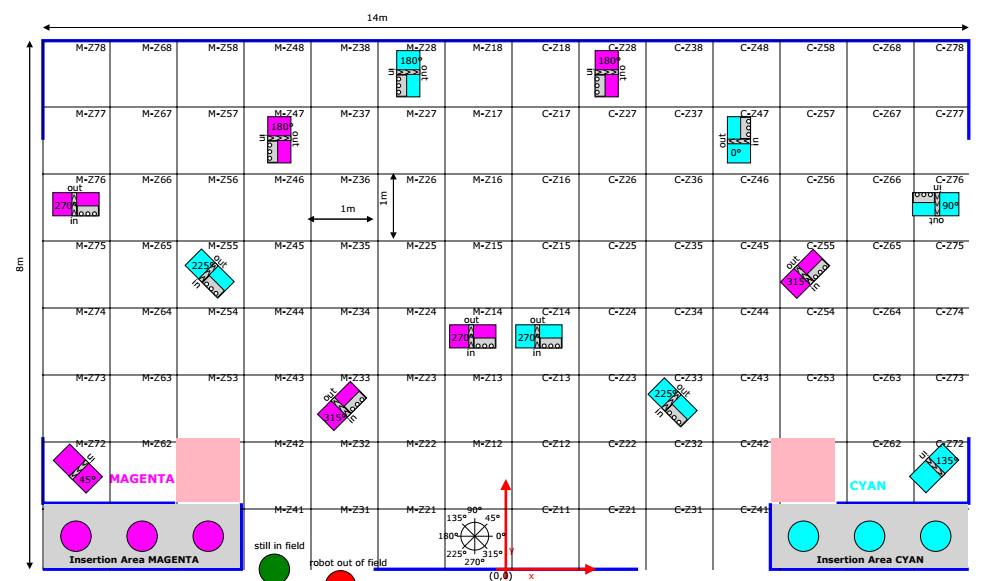
\includegraphics[width=\linewidth]{pic/field.png}
\caption{Field for robocup 2017}
\label{fig:frog}
\end{figure}

\subsection{Difficulties}

Some difficulties have been faced because the Smartbots team has been informed of the new rules during the Robocup. First, it was needed to implement a way to explore field without previous knowledge about the position due to the change in the Rulebook. To face this, a path has been created with some fixed zone in the instruction planer component.  Then, it was necessary to get the zone and the orientation of a detected MPS. This task has not been fulfilled for the Robocup. The last difficulty was to set up the network. There were two configurations, one to test and one to participate to the match.
 

\subsection{Situation in the Robocup}

To conclude, the team could accomplish some actions. First, only one robot was moving for each match because there was not multi-deployment. To do the exploration phase, the robot was going in some fixed positions (landmarks). There was no detection of the zone and the orientation of a MPS however the Alvar tag detection was fully working. The production phase was not implemented and the maintenance phase was not handled. The communication between all component (Refbox Server, Instruction planer, Alvar Tag detection and MPS docking was working and complete. 

\section{Components}

\subsection{Overview}
	This chapter shall give an overview of the current states of the particular components including the SmartAlvarTagDetection, the SmartRobotinoInstructionPlanner, the Refbox and the SmartMPSDocking components. Each chapter gives an insight on how the component works, how the component is modelled, tested and integrated in the masterdeployment
	
\subsection{SmartAlvarTagDetection}
	 \subsubsection{Overview}


This section is about the SmartAlvarTagDetection Component. The component is used to identify the Alvar Tags on the MPS machines, which is required for the exploration phase where the robots have to explore the game field and find MPS machines and identify the MPS based on their Alvar Tag. \\

Each MPS has their own Alvar Tag, one in the front and one in the back of the machine. This is important for the production phase later. On the field there are seven machines for each team. There are four types of MPS Machines, Base station, Cap station, Ring station and Storage station. All together there are 14 machines with 28 Alvar Tags. \\
Bild von Alvar Tag auf einer MPS. \\

The main idea is that the SmartAlvarTagDetection component identifies the tags. To do so, the component uses an algorithm to determine the Alvar Tag. Therefore, the component needs a picture of the Tag which is taken by a webcam mounted on each of the robotinos and operated by the SmartUnicapImageServer. The SmartAlvarTagDetection components is only one out of many components that are operated and instructed by the InstructionPlanner via the Sequencer (LISPServer). \\
Explain how to operate SmartAlvarTagDetection and SmartUnicapImageServer with DeploymentAlvarTagTest

\subsubsection{CommObjects}

This section describes the CommObjects that are used to communicate with the InstructionPlanner and other componentes.

\subsubsection{Previous State}

The team from the previous semester already had an implementation of the SmartAlvarTagDetection. In their version, they only had implemented the algorithm to scan pictures and identify whether there is a tag or not. They could not communicate with other components or the InstructionPlanner. \\

\begin{figure}[h]
\centering
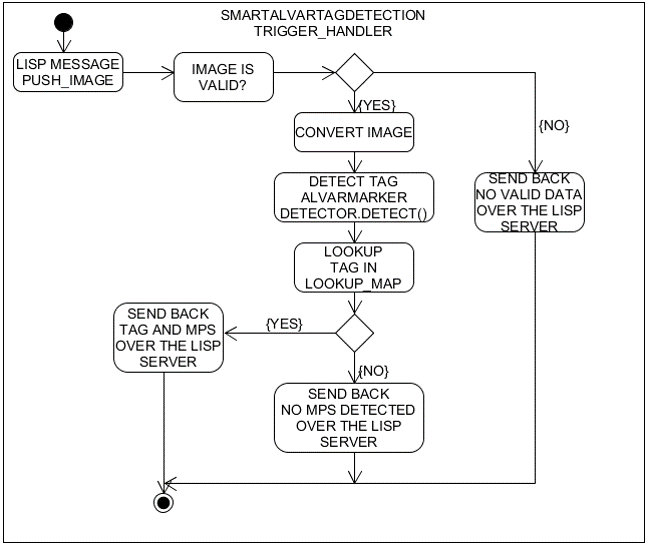
\includegraphics[scale=0.5]{pic/SmartAlvarTagDetectionFlow.png}
\caption{Describes the flow of the SmartAlvarTagDetection Trigger Handler}
\label{fig:smartAlvarFlow}
\end{figure}


At first, the SmartUnicapImageServer is being activated to take a picture and push an image to the SmartAlvarTagDetection. If the SmartUnicapImageServer is done, the LISP Server starts the SmartAlvarTagDetection Trigger Handler. The first thing the Trigger Handler does, is performing a validity check on the picture, to see if the picture can be used or not. If it is not valid, it returns a message saying that the image is not valid. But if it is valid, the image is converted into a greyscale picure, making it easier to recognize the Alvar Tags. Next, the marker detector has to detect an Alvar Tag on the image. It determines the ID by detecting and scanning the tag. In a lookup table this ID is searched and if there is a tag belonging to the ID, then this marker is returned. Markers consist of the type of station, the side and the team color. If the ID cannot be found an error message is returned, otherwise a positive message is returned. \\
Bild von Lookup table \\

The main Problem in this approach was the weak error handling. When for instance no ID could be found on the image and therefore the lookup was not possible, then the entire Robotino crashed. Another problem was that there was no proper communication with the SmartRobotinoInstructionPlanner. When the MPS was detected and found in the lookup table, the positive message was directly sent to the RefBoxServer and not to the SmartRobotinoInstructionPlanner. The communication flow was not transparent. Another problem, not with the implementation but rather with the Alvar and OPENCV libraries, was that it only was possible to deploy the SmartAlvarTagDetection on one computer. Due to difficulties of installing the libraries.



\subsubsection{Current State}

The current version, which was used in the 2017 RoboCup German Open Logistics Leauge in Magdeburg, is able to identify the tags, communicate with the InstructionPlanner via the LISP Server and has some sort of error handling. When the SmartAlvarTagDetection returns the message, that no tag was found, the InstructionPlanner keeps triggering the component five times and if it still sends no tag was found, one can be sure that there really is no tag and it is not a problem with the algorithm or bad picture quality. \\

\begin{figure}[h]
\centering
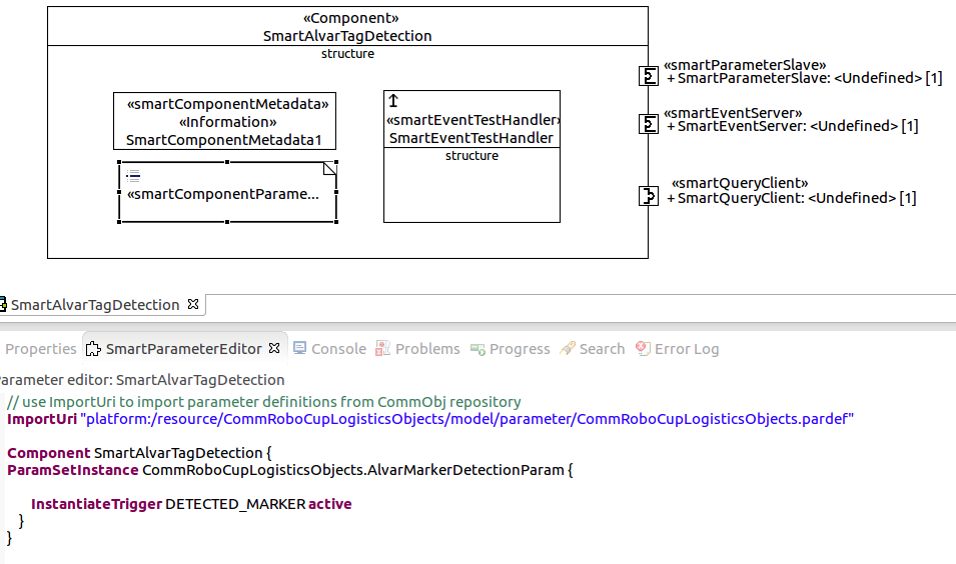
\includegraphics[scale=0.5]{pic/DeploymentAlvarTag.png}
\caption{Shows the model of the SmartAlvarTagDetection component}
\label{fig:smartAlvarFlow}
\end{figure}



The current model consists of a smartEventServer port, a smartQueryClient port and a smartParameterSlave port, but described will be only the first two. The smartEventServer is connected to the LISP Servers' visualMarkerEventClient, which is used to trigger the SmartAlvarTagDetection Trigger Handler.
The other is the SmartQueryClient which is connected to the SmartUnicapImageServers' imageQueryServer to push images that are taken by the webcam to the SmartAlvarTagDetection. The other noticable thing is the smartComponentParameter, which defines the behavior of the SmartAlvarTagDetection component to a Trigger behavior. The smartEventTestHandler is used to check whether an Event fires accordingly. In this case, it tests whether the correct MarkerDetectionState has been set. MarkerDetectionStates are the detected MPS as states. For instance, the tag with ID = 1 has been detected, then the MarkerDetectionState is set to MARKER CYAN CAP STATION 1 FRONT.

	
\subsection{SmartRobotinoInstructionPlanner}
	This is the InstructionPlanner

test for commiting


\subsection{Refbox}
	
\subsubsection{General}

The Referee Box (Refbox) is an external component build by Aachen University. This component controls, monitors, and evaluates the game during the Robocup. It communicates with robots of both teams and the MPS, attributes the points and manages the different phases of the game. To get more information, it is recommended to read the referee box manual located at \url{http://www.robocuplogistics.org/refbox}. To parametrize the Refbox, the file “config.yaml” should be modify. The most important part to change inside this file is the ip addresses.
 

\subsubsection{Old situation}

There was no permanent Refbox installed in the laboratory. Each team was forced to install on PC in the lab or on his own computer a Refbox with all necessary libraries.


\subsubsection{Current situation}

During this year, a permanent Refbox with all the necessary libraries for the Robocup 2017 version (tneumann/rcll17) have been installed on an independent laptop. Any person that need to test situations with the Refbox can take easily the laptop near his computer or access with XTightVncViewer.  To do this, it is necessary to run the server on the laptop with the command “tightvncserver”. Then it possible to access with the command “xtightvncviewer <<ipAdress>> :1”.  In the current network, the ip address was “172.26.1.112”. The Refbox changes regularly so it is necessary to update each new stable version of the Refbox. All versions can be seen with this link: https://git.fawkesrobotics.org/llsf-refbox.git. A contact with Tim Niemueller, one of the main developer of the Refbox, should be established to know the good version.


\subsubsection{Difficulties}

During the Robocup 2017, some difficulties have been faced. First, it is not possible to choose a zone for a MPS with the Refbox. It results that a successful test is more difficult to do in a smaller area. With this problem, we have use only check if the Refbox can detect the MPS report from robotinos. We were not interested by a correct report. Indeed, there are not MPS in the center of the field with the current generation done by the Refbox. Another problem was to get the last version of the Refbox. Indeed, the current version in the trunk during the Robocup was the Refbox 2016. It was needed to search in a branch to find the correct version of the Refbox. The setting of the network was not easy during the Robocup.



\subsection{SmartLogisticsRefboxServer}
	
\subsubsection{Overview}

This component is the interface for the Refbox. It handles the communication between the Refbox and the robotinos. Without this, it is not possible to know the phase of the game and to earn points. \\

This component is the key element for handling the communication between the referee box and the robotinos. Its functionality is very important, since communication to the referee box is essential to receive game instructions and report sensed information to gain points. If you need a full understanding of the communication patterns, it is recommended to read also the referee box manual located at \url{ http://www.robocup-logistics.org/refbox}. It describes the used protobuf (\url{https://developers.google.com/protocol-buffers}) messages in a detailed way. In the current state, the component covers most of the use cases needed for the Robocup competition.
 

\subsubsection{Situation in 2016}

//reference to the technical report from the previous team \\

In the old version of the code, the RefBox Server component was not used to send back information about detected MPS. So, there was no complete communication with InstructionPlaner and Refbox. There was not Refbox installed in the laboratory. 


\subsubsection{Situation in 2017}

About the Refbox server component, some new objects need to be handle (new zones, new MPS) that's why some communication objects have been added. Getting from the Refbox the team color and current game phase is working and tested. Send color and phase to InstructionPlaner component is also working. The detection of the maintenance phase is now possible. Send MPS information like zones, orientation from Refbox server to Refbox is working. The Refbox adds successfully points for good MPS reports and remove points for wrong MPS reports. It is necessary to modify the following parameters: the \textbf{HostIP} which is the IP address of the referee box, the \textbf{Name} which represent the name of the robotino (this name will be listed at the referee box GUI), the \textbf{Number} which is the (jersey) number of the robotino (this number will be listed at the referee box GUI) and the \textbf{Cryptokey} which is the key used for encrypted team channel.\\

\subsubsection{Classes}

//maybe show some graphics here \\
//deployment or class diagram  \\
//sequence charts  \\
//something like this \\

//i used lucidchart.com for diagrams \\

There are several classes in Refbox Server component. Each class will be described here. Reading the source code at the same time is recommended.\\

First, the \textbf{RefboxPeer} class owns the instances of protobuf peers. One peer is created for the team channel and another one for the public channel. The peers are used to receive and send protobuf messages via the corresponding channels. Note that our robots never send via the public channel but only listen to it. All used protobuf messages must be registered into the peer’s message register. To handle all received messages, the peers are connected to a signal handler, which is represented by the class \textbf{CommunicationHandler}. \\

Next, the \textbf{CommunicationHandler} class permit to trigger the handle message method when a message is received from a connected peer. Depending on the type of the message, a specific evaluation method of the \textbf{MessageEvaluator} class is called to decode the message.\\

Then, the \textbf{MessageEvaluator} class has an overloaded method named evaluate which is applied for any kind of message type. However, not all of the overloaded variants have been implemented so far. Until now, only the relevant message types needed for the exploration phase are completely realised (GameState and ExplorationInfo). Each variant is supposed to read the protobuf message and to extract the most important information into the internal communication objects of type CommRefbox. Those are used to pass the relevant information to the instruction planner component. For the production phase, the evaluate method for the orderInfo message has to be developed.\\

Next the \textbf{ConnectionMaintenance} class has a task which send a beacon signal every two seconds via the team peer. This is the periodic heartbeat signal to the referee box, which makes the referee box aware of the robots’ presence. Therefore, also some information of the robot is contained in the message, such as its name, team name and number.\\

Finally, the \textbf{PeerCommunication} class is the component’s smartTask of the SmartSoft environment. This means this is the loop construct which will be run as long as the component is active. At the current state, it does nothing more than sending new registered information about the gamestate or explorationinfo messages to the instruction planner via the push server.\\


\subsubsection{Difficulties}

About the Refbox server, the encryption was different in the competition and in the laboratory. An Electronic Code Book (ECB) was needed in Robocup and Cipher Block Chaining (CBC) is used with the Refbox installed in the laboratory. \\

//Maybe improve grammar and spelling ;) 
	
\subsection{SmartMPSDockingRobocup}
	This is the MPSDockingDetection

\printbibliography

\end{document}